This student report is written as part of a learning project. Therefore we must comply with the study regulation.

The study regulation states that the main focus of this semester's project is to gain knowledge of, and develop: Internet applications, -agents, or -services.
The goal is thus to create an Internet application that provides a service with focus on agent technologies, scalability, and data intensity.

\section{Motivation}
When a crime occurs documentation is often needed in order to convict the person(s) responsible and to receive repairs from an insurance company for the damages suffered.
Documentation can be eye witnesses, forrensic evidence, or video surveillance.
Documentation in the form of eye witnesses and forensic evidence is unreliable, as it is not possible to guarentee it will be available.
Video surveillance is however always obtainable, but it is far from a perfect solution in its current form.\fixme{Statement - source}

\subsection{Video Surveillance}
Video surveillance is widely used to obtain documentation or evidence of a crime, or as a preventive tool.
As an example there is one camera for every 32 people in the United Kingdom\citep{london_camera_surveillance}.
This number includes both cameras installed by the government to surveil London, but also cameras installed by businnes to secure their property.
The high number of cameras is partially attributed to the high need for surveillance to prevent e.g. terrorist attacks in London, but additionally due to the technical difficulties of video surveillance.
A typical video surveillance solution consists of a set of cameras connected via cables to a ``command station''
Video cameras are mounted on a fixed location, and can therefore only surveil an area limited by their field of view, see Figure~\ref{fig:camera_properties}, and the environment in which it is placed.

\begin{figure}[htb]
    \centering
    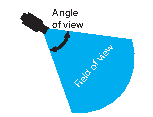
\includegraphics[scale=1.8]{gfx/camera_properties.pdf}
    \caption{A cameras field of view}
    \label{fig:camera_properties}
\end{figure}

An environment can contain physical objects which limits the cameras field of view further, see Figure~\ref{fig:refular_camera_setup}.
In small environment a sufficient degree surveillance can be achieved without too much difficulty or cost\fixme{Statement - source til prisetr evt.}.
Properly surveilling large areas, in particular outdoor changing environments, is however problematic.\fixme{ref til Lytzen}

\subsection{Video Surveillance of large Outdoor Areas}\label{subsec:surveillance_of_large_outdoor_areas}
%The need for video surveillance is based on the need for documentation of crimes, which is required in case of damage loses from an insurance perspective.
%Should a break-in occur a definitive proof of such must often be presented in order for insurances to cover potential losses.
<<<<<<< HEAD
Similarly video footage or witnesses is in most cases required in order to convict a person of a break-in.
One solution to the problem is to have mounted video cameras.
Video cameras have a limited scope, both in terms of view angle and distance, in order for the quality to be suited for documentation.
This limitation can make it tough, and very resource intensive to surveil large areas.
The resource intensitivity stems from the amount of hardware required to surveil in terms of cameras, and cables connecting the surveillance system.
There are two types of environments regarding real-world surveillance; indoor and outdoor.
Outdoor surveillance has the unpredictable variables: weather and airspace.
The weather has several parameters that constitute to the environment e.g. wind, fog, rain, sun.
The outdoor airspace is in general larger outdoor, but less well-defined.
A well-defined environment is an environment that is predictable and bounded.
Both indoor and outdoor pose challenges e.g. objects being moved around and blind spots.
=======
%Similarly video footage or witnesses is in most cases required in order to convict a person of a burglary.
%One solution to the problem is to have mounted video cameras.
Video cameras have a limited field of view, both in terms of vision and range, and only within this field of view is the quality high enough be usable as documentation.
This limitation can make it difficult and resource intensive to surveil large areas.
The resource intensitivity stems from the amount of hardware required to surveil, referring to both cameras, and the cables needed to connect the surveillance system.
The difficulty in surveilling the areas comes from the nature of an outdoor environment.
In terms of surveillance an indoor environment is static, as there is a limited amount of entrances and the interior of the buildings in terms of walls and doors remain the same.
In an outdoor environment the weather has to be taken into account.
The weather can be foggy, rainy, and the sun can blind a camera if it is improperly placed.
These conditions makes video surveillance of outdoor areas difficult.
Both indoors and outdoors does however have some challenges that needs to be faced, such as physical objects being moved around creating blind spots etc.
>>>>>>> 546af54017f7407930718fc28281185cf976bea6

\subsection{Current solutions}
This section will discuss the current solutions used for video surveillance.
The strengths and weaknesses of each solution will be covered.
The figures referenced in this section show the same area with a different surveillance setup to make them comparable.
\subsubsection{Regular camera solution}
In a regular camera solution mounted cameras are used.
These cameras surveil a limited area, and in order to cover a larger area, multiple cameras are needed.
With multiple cameras multiple areas are surveilled simultaneously.
A limitation with a regular camera setup, is that the cameras are stationary.
This means a cameras field of view can be limited by physical objects.
As an example in Figure~\ref{fig:refular_camera_setup} it can be seen how an object placed in a cameras field of view can create a blind spot in an area normally covered by a camera.
\begin{figure}[htb]
    \centering
    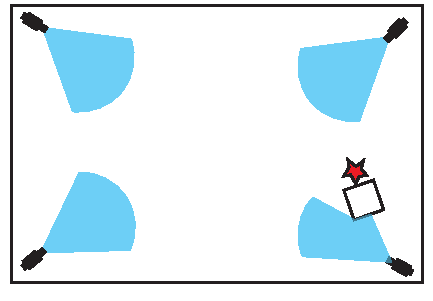
\includegraphics[width=\textwidth]{gfx/regular_camera_setup.pdf}
    \caption{An Example of a Regular Camera Setup}
    \label{fig:refular_camera_setup}
\end{figure}
The red star in Figure ~\ref{fig:refular_camera_setup} represents a critical object, that needs to be observed.

\subsubsection{Photo Sensor Camera Solution}
In a photo sensor solution the perimeter of the surveilled area is covered by both cameras and photo sensors.
The purpose of the setup is to detect if anything enters the area, and then activate the cameras to capture it on video, as seen in Figure~\ref{fig:photo_sensor}.
A photo sensor solution can be used in combination with a regular camera solution, to surveil both the interior and the perimeter of an area.
The advantage of a photo sensor setup is that the cameras surveilling the perimeter are only activated if the sensors are triggered, ensuring video footage is only recorded when it is needed.
The disadvantage is that the cameras are still stationary, meaning the a large amount of cameras are required to surveil a large area.
\begin{figure}[htb]
    \centering
    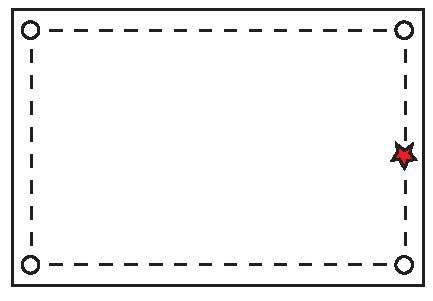
\includegraphics[width=\textwidth]{gfx/light_sensor.pdf}
    \caption{A Photo Sensor Setup}
    \label{fig:photo_sensor}
\end{figure}

\subsubsection{Dome camera solution}
This solution centers around having a dome camera with a long field of view in the center.
The perimeter is then divided into zones, by fx. light sensors.
When a zone have detected an entry, the dome camera is rotated towards that zone to observe the area.
Compared to the two previous solution, the dome camera solution is limited to only observe a specific subarea at a time, as seen in Figure~\ref{fig:drone_sensor}.
\begin{figure}[htb]
    \centering
    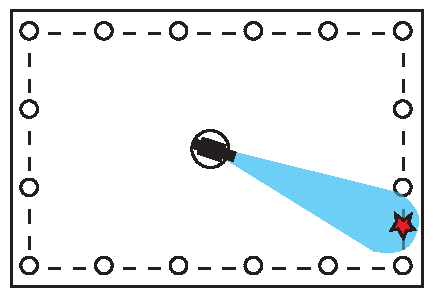
\includegraphics[width=\textwidth]{gfx/drome_sensor.pdf}
    \caption{A Dome Setup}
    \label{fig:drone_sensor}
\end{figure}

\subsection{Moveable Cameras}
As mentioned in Section~\ref{subsec:surveillance_of_large_outdoor_areas} the main problems with surveillance is the ammount of hardware required, particularly cables, and the limited field of view of cameras.
A possible solution is to switch from fixed cameras to movable cameras.
A movable camera is one capable of moving freely in the environment it is to surveil.
This can be achieved with the use of drones with an onboard camera.
A drone in this context is a pilotless aircraft controlled via remote controll.
Drones capable of moving freely in an environment is capable of surveilling a larger area with fewer cameras, than a traditional setup, and they remove the problem with blind spots.
The need for cables is also removed by using drones, as they are typically controlled using wireless internet technologies or radio waves\fixme{source}.

\subsection{Internet Technologies in a Surveillance Perspective}
With the development and standardization of network technologies, video surveillance is becoming digitized.
The digitization of video surveillance is important as it e.g. makes it faster to examine a video recording, and video cameras can be programmed to trigger alarms when they detect movement.
Video recordings are examined faster as it is easy to skip through digital data compared to the analog data which would be stored on e.g. a VHS cassette.
The programming of video cameras is possible due to the data being digital. 
It is possible to apply algorithms to examine the digital Sdata, which could e.g. identify license plates.
The digitization allows for the use of the internet.
The internet makes it possible to interconnect surveillance solution, that enables features such as backup or long distance observing.








%In their current form most security systems consist of a set of sensors and cameras, each covering a limited area.
%Both a sensor and a camera is limited by its range and spectrum.
%As a consequence security systems require a large amount of hardware to monitor a large area to a satisfying degree.
%Hardware is expensive and therefore the cost of....
%However such a surveillance system still suffer from most of its hardware components being static.
%This means that if a sensor is triggered in an area not covered by a camera, a security company would have to send a guard to the location to investigate the source of the alarm.
%The static nature of security systems combined with the high costs security guards makes it very expensive for a company to properly secure their property.\footnote{Sources for this section, pretty important}

%A possible solution to the high cost and static nature of security systems could be a non-static and self movable surveillance system where cameras are placed on a drone capable of flight.
%In such a system a guard would be able to access and control a drone through a web application to investigate what triggered an alarm, and based on a video stream determine whether or not to send someone to the location.
%Moveable cameras would reduce the amount of hardware required, and the manpower required to investigate alarms.
%Therefore the idea of a drone-based surveillance system is interesting to investigate.

%\subsection{}

%The goal of this project is to develop a drone-based surveillance system, in order to reduce economical cost and save manpower.


%Old: static (Both in terms of camereas and possibly the controlcenter), expensive, slow in response (Regular alarm systems).

%New: dynamic, controllable from a single source, possibly cheaper